\chapter{Simultaneous Localization and Planning}\label{chap:localization-and-planning}

\todo[inline]{Rework according to results}

Typically, robot localization and motion planning are treated as mostly
independent tasks. Often, the problem provides the agent with a focused initial
belief or allows the agent to quickly reduce uncertainty by first collecting
a series of measurements that don't require elaborate motion planning. This is
particularly the case if the state space is well observed, i.e. there exists
a sensor that provides the robot with a (noisy) position reading (e.g. GPS).
For these well behaved problems, a simple yet effective approach is to first
collect sensor data while executing a default motion, i.e. rotating about the
yaw axis to collect measurements in all directions. Once state uncertainty is
reduced to a focused, unimodal belief, the problem is treated as fully observed
problem and motion planning is performed on expectation. That is, trajectories
are planned based on the assumption that the expectation of the belief, $E[b]$,
is a sufficient approximation for the true position of the robot. Furthermore,
higher statistical moments \todo{What is the right word for this?} may be used
to trigger additional information gathering. In even simpler problems, plan
execution may implicitly yield sufficient information gathering, rendering
explicit consideration of this aspect obsolete.

However, more challenging problems are obtained when information gathering
happens less naturally. In these cases, a simple approach as outlined above
does not perform well. Instead, state estimation requires the agent to consider
the full belief distribution as well as future observations in order to
identify informative action sequences.


\todo[inline]{Rewrite once structure (below) has converged}
An instance of such problem is studied in this chapter. We begin by stating the
problem details in \cref{sec:lp-problem-statement}.
\cref{sec:lp-pomdp-formalization} then formalizes this problem as a \ac{pomdp}.
Finally, we solve this problem using the methods presented in
\cref{chap:fundamentals} to evaluate the performance against a base
line policy in \cref{sec:lp-evaluation}.

\section{Problem Statement}\label{sec:lp-problem-statement}

Consider a robot operating in a planar, previously mapped room as depicted in
\cref{fig:roomba-env}. In this figure the red marker denotes the true position
of the robot, while the blue particles represent the robot's belief of it's
current location in the room. The agent is tasked to reach the exit (green)
while avoiding falling down the stairs (red). Additionally, unnecessary
collisions are to be avoided. The scene shows the simulation in it's initial
configuration: The robot starts at a position drawn uniformly at random from
the set of all possible position-orientation tuples. This initial position is
not known by the agent, thus the particles representing the initial belief are
spread uniformly across the entire room. The robot is equipped with a single
sensor that provides information about collisions with walls of the room. The
robot's dynamics are governed by an underactuated first-order model that allows
the robot to translate forward and/or rotate about it's vertical axis. The
agent holds control authority tho choose translation and rotation rates,
respectively.

This problem has originally been published under the name \emph{"Escape
Roomba"} by the \emph{Stanford Intelligent Systems Laboratory} as part of the
class \emph{Decision Making under
Uncertainty}\footnote{\url{https://web.stanford.edu/class/aa228/cgi-bin/wp/}}.
The experiments presented in the following have been conducted in the
simulation environment provided by project\footnote{\url{https://github.com/sisl/AA228FinalProject}}.

\begin{figure}[htpb]
  \centering
  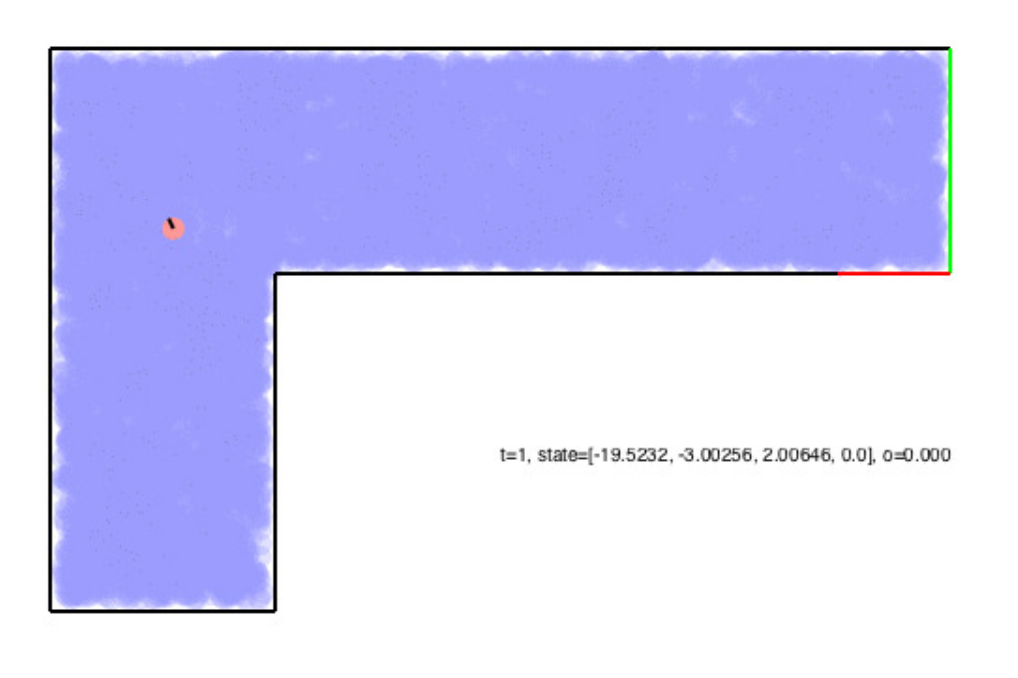
\includegraphics[width=0.7\textwidth]{roomba_demo/roomba-initial.png}
  \caption{A screen shot of the simulation environment for the \emph{"Escape
  Roomba"} problem provided by the \emph{Stanford Intelligent Systems
  Laboratory} as part of the class \emph{Decision Making under Uncertainty}.}
  \label{fig:roomba-env}
\end{figure}

\clearpage
\section{POMDP Formalization}\label{sec:lp-pomdp-formalization}

The problem is formalized as a \ac{pomdp} with the following properties introduced in \cref{sec:pomdp}:

\begin{description}
	\item[State Space $\sspace$.] The state of the robot is defined as the
	position, orientation tuple, $s=((x,y), \alpha)$. Respectively, $\sspace$ is
	the set of all positions-orientation tuples inside the room.
	\item[Action Space $\aspace$.] An action is defined as a translation-rotation
		rate tuple, $a=(v, \omega)$. $\aspace$ is the set of all these
		tuples adhering to the physical limitations of the system.
  \item[Transition Model $\tdist$.] The robot transition flows the dynamics of
    a simple differential drive model. The details of this transition are
    defined implicitly by the simulator and are treated as a generative black
    box model.
  \item[Reward Function $\reward: \sspace \times \aspace \times
    \sspace \to \reals$.] The reward model is defined as:
    \begin{equation}
      \reward(s, a, s') = r_\text{time} + \chrond(s') r_\text{collision} + \chrond(s') r_\text{goal} + \chrond(s') r_\text{stairs}.
    \end{equation}
    Here, $\chrond_\text{c}(s)$ denotes the \vname{Kronecke delta} function under the condition, \vname{c}, such that
    \begin{equation}
      \chrond_\text{c}(s) = \begin{cases}
        1, & \text{if condition $c$ holds for $s$}\\
        0, & \text{otherwise.}
      \end{cases}
    \end{equation}
    The reward model is parametrized by the following
    quantities: $r_\text{time}$ is a living penalty encouraging the robot to
    minimize the time until the goal is reached; $r_\text{collision}$ is
    a penalty for collision with walls; $r_\text{goal}$ is the reward obtained
    when reaching the goal, and $r_\text{stairs}$ the penalty for falling down
    the stairs.\\
  \item[Discount Factor $\gamma$.] Rewards are discounted with $\gamma = 0.99$.
  \item[Observation Space $\ospace$.] The sensor provides a binary output,
    stating whether the robot is currently in contact with the wall or not. That
    is, there are only two observations: $o^0$  and $o^1$.
  \item[Observation Model $\odist$.] The collision sensor is deterministic.
    That is, the observation model is a Dirac delta function, evaluating
    non-zero for a state, $s$, if and only if the collision feature evaluated
    on $s$ matches the observation, $o$.
\end{description}

Summarizing, the problem is a \ac{pomdp} with continuous state and action space
and a discrete observation space. The reward model chosen for this problem is
sparse. That is, it only encodes high level preferences but avoids biasing the
solution through additional transition dependent rewards (e.g. rewards for
reducing the distance to the goal).

\section{Solution Strategies}\label{sec:lp-solutions}

\subsection{Base Line}\label{sec:lp-baseline}

\subsection{POMDP Solutions}\label{sec:lp-planners}

\section{Evaluation}\label{sec:lp-evaluation}
